\documentclass[twoside]{book}

% Packages required by doxygen
\usepackage{fixltx2e}
\usepackage{calc}
\usepackage{doxygen}
\usepackage[export]{adjustbox} % also loads graphicx
\usepackage{graphicx}
\usepackage[utf8]{inputenc}
\usepackage{makeidx}
\usepackage{multicol}
\usepackage{multirow}
\PassOptionsToPackage{warn}{textcomp}
\usepackage{textcomp}
\usepackage[nointegrals]{wasysym}
\usepackage[table]{xcolor}

% Font selection
\usepackage[T1]{fontenc}
\usepackage[scaled=.90]{helvet}
\usepackage{courier}
\usepackage{amssymb}
\usepackage{sectsty}
\renewcommand{\familydefault}{\sfdefault}
\allsectionsfont{%
  \fontseries{bc}\selectfont%
  \color{darkgray}%
}
\renewcommand{\DoxyLabelFont}{%
  \fontseries{bc}\selectfont%
  \color{darkgray}%
}
\newcommand{\+}{\discretionary{\mbox{\scriptsize$\hookleftarrow$}}{}{}}

% Page & text layout
\usepackage{geometry}
\geometry{%
  a4paper,%
  top=2.5cm,%
  bottom=2.5cm,%
  left=2.5cm,%
  right=2.5cm%
}
\tolerance=750
\hfuzz=15pt
\hbadness=750
\setlength{\emergencystretch}{15pt}
\setlength{\parindent}{0cm}
\setlength{\parskip}{3ex plus 2ex minus 2ex}
\makeatletter
\renewcommand{\paragraph}{%
  \@startsection{paragraph}{4}{0ex}{-1.0ex}{1.0ex}{%
    \normalfont\normalsize\bfseries\SS@parafont%
  }%
}
\renewcommand{\subparagraph}{%
  \@startsection{subparagraph}{5}{0ex}{-1.0ex}{1.0ex}{%
    \normalfont\normalsize\bfseries\SS@subparafont%
  }%
}
\makeatother

% Headers & footers
\usepackage{fancyhdr}
\pagestyle{fancyplain}
\fancyhead[LE]{\fancyplain{}{\bfseries\thepage}}
\fancyhead[CE]{\fancyplain{}{}}
\fancyhead[RE]{\fancyplain{}{\bfseries\leftmark}}
\fancyhead[LO]{\fancyplain{}{\bfseries\rightmark}}
\fancyhead[CO]{\fancyplain{}{}}
\fancyhead[RO]{\fancyplain{}{\bfseries\thepage}}
\fancyfoot[LE]{\fancyplain{}{}}
\fancyfoot[CE]{\fancyplain{}{}}
\fancyfoot[RE]{\fancyplain{}{\bfseries\scriptsize Generated by Doxygen }}
\fancyfoot[LO]{\fancyplain{}{\bfseries\scriptsize Generated by Doxygen }}
\fancyfoot[CO]{\fancyplain{}{}}
\fancyfoot[RO]{\fancyplain{}{}}
\renewcommand{\footrulewidth}{0.4pt}
\renewcommand{\chaptermark}[1]{%
  \markboth{#1}{}%
}
\renewcommand{\sectionmark}[1]{%
  \markright{\thesection\ #1}%
}

% Indices & bibliography
\usepackage{natbib}
\usepackage[titles]{tocloft}
\setcounter{tocdepth}{3}
\setcounter{secnumdepth}{5}
\makeindex

% Hyperlinks (required, but should be loaded last)
\usepackage{ifpdf}
\ifpdf
  \usepackage[pdftex,pagebackref=true]{hyperref}
\else
  \usepackage[ps2pdf,pagebackref=true]{hyperref}
\fi
\hypersetup{%
  colorlinks=true,%
  linkcolor=blue,%
  citecolor=blue,%
  unicode%
}

% Custom commands
\newcommand{\clearemptydoublepage}{%
  \newpage{\pagestyle{empty}\cleardoublepage}%
}

\usepackage{caption}
\captionsetup{labelsep=space,justification=centering,font={bf},singlelinecheck=off,skip=4pt,position=top}

%===== C O N T E N T S =====

\begin{document}

% Titlepage & ToC
\hypersetup{pageanchor=false,
             bookmarksnumbered=true,
             pdfencoding=unicode
            }
\pagenumbering{alph}
\begin{titlepage}
\vspace*{7cm}
\begin{center}%
{\Large Marshall\textquotesingle{}s Algorithms and Data Structures }\\
\vspace*{1cm}
{\large Generated by Doxygen 1.8.14}\\
\end{center}
\end{titlepage}
\clearemptydoublepage
\pagenumbering{roman}
\tableofcontents
\clearemptydoublepage
\pagenumbering{arabic}
\hypersetup{pageanchor=true}

%--- Begin generated contents ---
\chapter{Class Index}
\section{Class List}
Here are the classes, structs, unions and interfaces with brief descriptions\+:\begin{DoxyCompactList}
\item\contentsline{section}{\mbox{\hyperlink{structCAPHStruct}{C\+A\+P\+H\+Struct}} }{\pageref{structCAPHStruct}}{}
\item\contentsline{section}{\mbox{\hyperlink{structcorrHelpStructBruteForce}{corr\+Help\+Struct\+Brute\+Force}} }{\pageref{structcorrHelpStructBruteForce}}{}
\item\contentsline{section}{\mbox{\hyperlink{structcorrHelpStructCrossReference}{corr\+Help\+Struct\+Cross\+Reference}} }{\pageref{structcorrHelpStructCrossReference}}{}
\item\contentsline{section}{\mbox{\hyperlink{structEnhancedSuffixArray}{Enhanced\+Suffix\+Array}} }{\pageref{structEnhancedSuffixArray}}{}
\item\contentsline{section}{\mbox{\hyperlink{structEnhancedSuffixArrayCaster}{Enhanced\+Suffix\+Array\+Caster}} }{\pageref{structEnhancedSuffixArrayCaster}}{}
\item\contentsline{section}{\mbox{\hyperlink{structGeoSoft}{Geo\+Soft}} }{\pageref{structGeoSoft}}{}
\item\contentsline{section}{\mbox{\hyperlink{structGeoSoftChannel}{Geo\+Soft\+Channel}} }{\pageref{structGeoSoftChannel}}{}
\item\contentsline{section}{\mbox{\hyperlink{structmultithreadLoad}{multithread\+Load}} }{\pageref{structmultithreadLoad}}{}
\item\contentsline{section}{\mbox{\hyperlink{structrankHelpStruct}{rank\+Help\+Struct}} }{\pageref{structrankHelpStruct}}{}
\item\contentsline{section}{\mbox{\hyperlink{structSparseBitArrayRecord}{Sparse\+Bit\+Array\+Record}} }{\pageref{structSparseBitArrayRecord}}{}
\item\contentsline{section}{\mbox{\hyperlink{structSparseBitpackedArray}{Sparse\+Bitpacked\+Array}} }{\pageref{structSparseBitpackedArray}}{}
\item\contentsline{section}{\mbox{\hyperlink{structSuffixArray}{Suffix\+Array}} }{\pageref{structSuffixArray}}{}
\item\contentsline{section}{\mbox{\hyperlink{structSuffixArrayCaster}{Suffix\+Array\+Caster}} }{\pageref{structSuffixArrayCaster}}{}
\item\contentsline{section}{\mbox{\hyperlink{structtauCorrHelpStructBruteForce}{tau\+Corr\+Help\+Struct\+Brute\+Force}} }{\pageref{structtauCorrHelpStructBruteForce}}{}
\item\contentsline{section}{\mbox{\hyperlink{structtauCorrHelpStructCrossReference}{tau\+Corr\+Help\+Struct\+Cross\+Reference}} }{\pageref{structtauCorrHelpStructCrossReference}}{}
\item\contentsline{section}{\mbox{\hyperlink{structyy__buffer__state}{yy\+\_\+buffer\+\_\+state}} }{\pageref{structyy__buffer__state}}{}
\item\contentsline{section}{\mbox{\hyperlink{structyy__trans__info}{yy\+\_\+trans\+\_\+info}} }{\pageref{structyy__trans__info}}{}
\item\contentsline{section}{\mbox{\hyperlink{unionyyalloc}{yyalloc}} }{\pageref{unionyyalloc}}{}
\item\contentsline{section}{\mbox{\hyperlink{structyyguts__t}{yyguts\+\_\+t}} }{\pageref{structyyguts__t}}{}
\item\contentsline{section}{\mbox{\hyperlink{structYYLTYPE}{Y\+Y\+L\+T\+Y\+PE}} }{\pageref{structYYLTYPE}}{}
\item\contentsline{section}{\mbox{\hyperlink{unionYYSTYPE}{Y\+Y\+S\+T\+Y\+PE}} }{\pageref{unionYYSTYPE}}{}
\end{DoxyCompactList}

\chapter{Class Documentation}
\hypertarget{structCAPHStruct}{}\section{C\+A\+P\+H\+Struct Struct Reference}
\label{structCAPHStruct}\index{C\+A\+P\+H\+Struct@{C\+A\+P\+H\+Struct}}


Collaboration diagram for C\+A\+P\+H\+Struct\+:\nopagebreak
\begin{figure}[H]
\begin{center}
\leavevmode
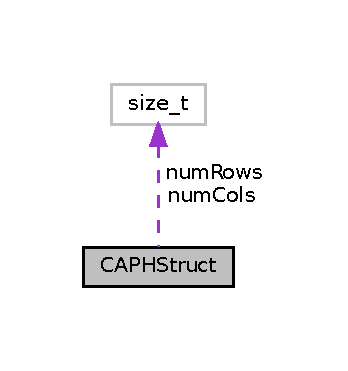
\includegraphics[width=167pt]{structCAPHStruct__coll__graph}
\end{center}
\end{figure}
\subsection*{Public Attributes}
\begin{DoxyCompactItemize}
\item 
\mbox{\Hypertarget{structCAPHStruct_a76219a6222c8003950c5585143ebfc5b}\label{structCAPHStruct_a76219a6222c8003950c5585143ebfc5b}} 
cf64 $\ast$$\ast$ {\bfseries expression\+Data}
\item 
\mbox{\Hypertarget{structCAPHStruct_a6515a128c8b5c23c91b5014785591a3d}\label{structCAPHStruct_a6515a128c8b5c23c91b5014785591a3d}} 
csize\+\_\+t {\bfseries num\+Rows}
\item 
\mbox{\Hypertarget{structCAPHStruct_a7f7c79a59b113eddd70e70b4712163b7}\label{structCAPHStruct_a7f7c79a59b113eddd70e70b4712163b7}} 
csize\+\_\+t {\bfseries num\+Cols}
\item 
\mbox{\Hypertarget{structCAPHStruct_ae431f8d57ef33b038493e9d549bbe133}\label{structCAPHStruct_ae431f8d57ef33b038493e9d549bbe133}} 
f64 $\ast$ {\bfseries sums\+Of\+Squares}
\end{DoxyCompactItemize}


The documentation for this struct was generated from the following files\+:\begin{DoxyCompactItemize}
\item 
src/pearson-\/correlation-\/matrix.\+cpp\item 
src/weighted-\/rank-\/correlation-\/matrix.\+cpp\end{DoxyCompactItemize}

\hypertarget{structcorrHelpStructBruteForce}{}\section{corr\+Help\+Struct\+Brute\+Force Struct Reference}
\label{structcorrHelpStructBruteForce}\index{corr\+Help\+Struct\+Brute\+Force@{corr\+Help\+Struct\+Brute\+Force}}


Collaboration diagram for corr\+Help\+Struct\+Brute\+Force\+:\nopagebreak
\begin{figure}[H]
\begin{center}
\leavevmode
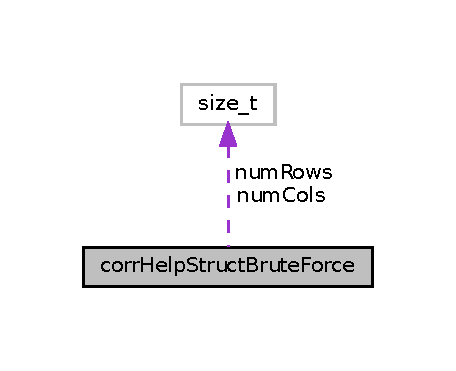
\includegraphics[width=219pt]{structcorrHelpStructBruteForce__coll__graph}
\end{center}
\end{figure}
\subsection*{Public Attributes}
\begin{DoxyCompactItemize}
\item 
\mbox{\Hypertarget{structcorrHelpStructBruteForce_af39d58f3d09b7ad663f82af75521c37a}\label{structcorrHelpStructBruteForce_af39d58f3d09b7ad663f82af75521c37a}} 
cf64 $\ast$ {\bfseries sums\+Of\+Squares}
\item 
\mbox{\Hypertarget{structcorrHelpStructBruteForce_a09a788c0291943229b3540daeb8b4e5c}\label{structcorrHelpStructBruteForce_a09a788c0291943229b3540daeb8b4e5c}} 
cf64 $\ast$$\ast$ {\bfseries expression\+Data}
\item 
\mbox{\Hypertarget{structcorrHelpStructBruteForce_a645d896963ade023a1ff805724e0a2e1}\label{structcorrHelpStructBruteForce_a645d896963ade023a1ff805724e0a2e1}} 
csize\+\_\+t {\bfseries num\+Rows}
\item 
\mbox{\Hypertarget{structcorrHelpStructBruteForce_a37303b729c3b46e812efe834098f837a}\label{structcorrHelpStructBruteForce_a37303b729c3b46e812efe834098f837a}} 
csize\+\_\+t {\bfseries num\+Cols}
\item 
\mbox{\Hypertarget{structcorrHelpStructBruteForce_a899ff1d82082fa63faa08d297147f95a}\label{structcorrHelpStructBruteForce_a899ff1d82082fa63faa08d297147f95a}} 
Upper\+Diagonal\+Square\+Matrix$<$ f64 $>$ $\ast$ {\bfseries results}
\end{DoxyCompactItemize}


The documentation for this struct was generated from the following files\+:\begin{DoxyCompactItemize}
\item 
src/pearson-\/correlation-\/matrix.\+cpp\item 
src/weighted-\/rank-\/correlation-\/matrix.\+cpp\end{DoxyCompactItemize}

\hypertarget{structcorrHelpStructCrossReference}{}\section{corr\+Help\+Struct\+Cross\+Reference Struct Reference}
\label{structcorrHelpStructCrossReference}\index{corr\+Help\+Struct\+Cross\+Reference@{corr\+Help\+Struct\+Cross\+Reference}}


Collaboration diagram for corr\+Help\+Struct\+Cross\+Reference\+:\nopagebreak
\begin{figure}[H]
\begin{center}
\leavevmode
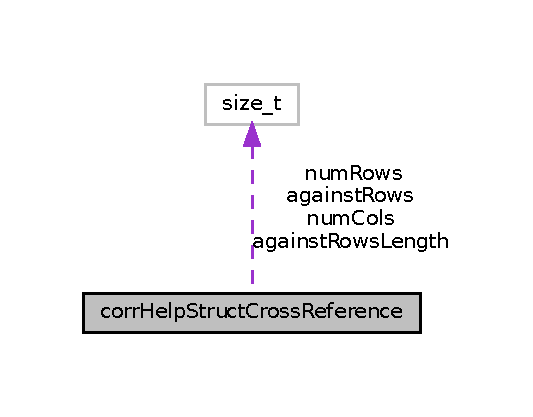
\includegraphics[width=256pt]{structcorrHelpStructCrossReference__coll__graph}
\end{center}
\end{figure}
\subsection*{Public Attributes}
\begin{DoxyCompactItemize}
\item 
\mbox{\Hypertarget{structcorrHelpStructCrossReference_aafd598ebfa0734685ae891ed2306b78d}\label{structcorrHelpStructCrossReference_aafd598ebfa0734685ae891ed2306b78d}} 
cf64 $\ast$ {\bfseries sums\+Of\+Squares}
\item 
\mbox{\Hypertarget{structcorrHelpStructCrossReference_a720074c2fe577537776bd423badbfd02}\label{structcorrHelpStructCrossReference_a720074c2fe577537776bd423badbfd02}} 
cf64 $\ast$$\ast$ {\bfseries expression\+Data}
\item 
\mbox{\Hypertarget{structcorrHelpStructCrossReference_a8915b3bf6686d0253996f3c6ec621c65}\label{structcorrHelpStructCrossReference_a8915b3bf6686d0253996f3c6ec621c65}} 
csize\+\_\+t {\bfseries num\+Rows}
\item 
\mbox{\Hypertarget{structcorrHelpStructCrossReference_af6ecc2f0e2191824f939747725f9edd1}\label{structcorrHelpStructCrossReference_af6ecc2f0e2191824f939747725f9edd1}} 
csize\+\_\+t {\bfseries num\+Cols}
\item 
\mbox{\Hypertarget{structcorrHelpStructCrossReference_a049d0b50801f8bea48034a80a376adf6}\label{structcorrHelpStructCrossReference_a049d0b50801f8bea48034a80a376adf6}} 
csize\+\_\+t $\ast$ {\bfseries against\+Rows}
\item 
\mbox{\Hypertarget{structcorrHelpStructCrossReference_a7f0def370016ca8e6702097caba1906c}\label{structcorrHelpStructCrossReference_a7f0def370016ca8e6702097caba1906c}} 
csize\+\_\+t {\bfseries against\+Rows\+Length}
\item 
\mbox{\Hypertarget{structcorrHelpStructCrossReference_ac43c5b1440fdeef2da8c5676918f56fa}\label{structcorrHelpStructCrossReference_ac43c5b1440fdeef2da8c5676918f56fa}} 
f64 $\ast$$\ast$ {\bfseries results}
\end{DoxyCompactItemize}


The documentation for this struct was generated from the following files\+:\begin{DoxyCompactItemize}
\item 
src/pearson-\/correlation-\/matrix.\+cpp\item 
src/weighted-\/rank-\/correlation-\/matrix.\+cpp\end{DoxyCompactItemize}

\hypertarget{structEnhancedSuffixArray}{}\section{Enhanced\+Suffix\+Array Struct Reference}
\label{structEnhancedSuffixArray}\index{Enhanced\+Suffix\+Array@{Enhanced\+Suffix\+Array}}


Collaboration diagram for Enhanced\+Suffix\+Array\+:\nopagebreak
\begin{figure}[H]
\begin{center}
\leavevmode
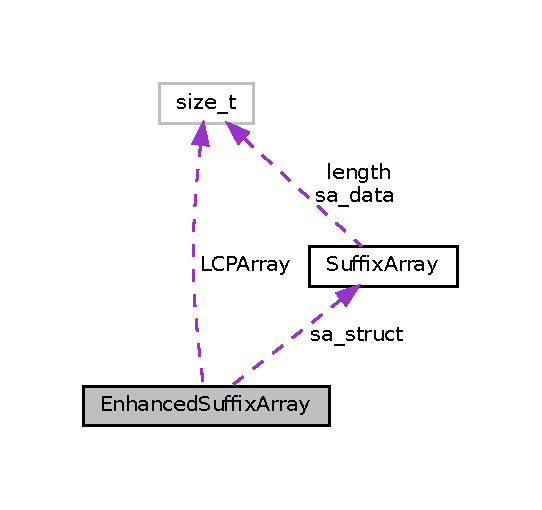
\includegraphics[width=260pt]{structEnhancedSuffixArray__coll__graph}
\end{center}
\end{figure}
\subsection*{Public Attributes}
\begin{DoxyCompactItemize}
\item 
\mbox{\Hypertarget{structEnhancedSuffixArray_a759e0da6c0567b61114606061bd07953}\label{structEnhancedSuffixArray_a759e0da6c0567b61114606061bd07953}} 
\mbox{\hyperlink{structSuffixArray}{Suffix\+Array}} {\bfseries sa\+\_\+struct}
\item 
\mbox{\Hypertarget{structEnhancedSuffixArray_a7e795867c7d43ef6f7a7b4f1963d45c2}\label{structEnhancedSuffixArray_a7e795867c7d43ef6f7a7b4f1963d45c2}} 
const size\+\_\+t $\ast$ {\bfseries L\+C\+P\+Array}
\end{DoxyCompactItemize}


The documentation for this struct was generated from the following file\+:\begin{DoxyCompactItemize}
\item 
include/matching.\+hpp\end{DoxyCompactItemize}

\hypertarget{structEnhancedSuffixArrayCaster}{}\section{Enhanced\+Suffix\+Array\+Caster Struct Reference}
\label{structEnhancedSuffixArrayCaster}\index{Enhanced\+Suffix\+Array\+Caster@{Enhanced\+Suffix\+Array\+Caster}}


Collaboration diagram for Enhanced\+Suffix\+Array\+Caster\+:\nopagebreak
\begin{figure}[H]
\begin{center}
\leavevmode
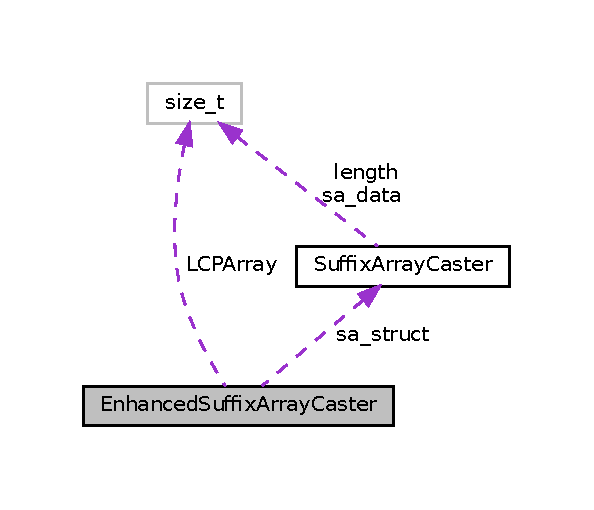
\includegraphics[width=285pt]{structEnhancedSuffixArrayCaster__coll__graph}
\end{center}
\end{figure}
\subsection*{Public Attributes}
\begin{DoxyCompactItemize}
\item 
\mbox{\Hypertarget{structEnhancedSuffixArrayCaster_acb3af842c32fba480dad8d0323e0923c}\label{structEnhancedSuffixArrayCaster_acb3af842c32fba480dad8d0323e0923c}} 
\mbox{\hyperlink{structSuffixArrayCaster}{Suffix\+Array\+Caster}} {\bfseries sa\+\_\+struct}
\item 
\mbox{\Hypertarget{structEnhancedSuffixArrayCaster_ab99fa020e1f4e2b2c3b9c08a3d65dc30}\label{structEnhancedSuffixArrayCaster_ab99fa020e1f4e2b2c3b9c08a3d65dc30}} 
size\+\_\+t $\ast$ {\bfseries L\+C\+P\+Array}
\end{DoxyCompactItemize}


The documentation for this struct was generated from the following file\+:\begin{DoxyCompactItemize}
\item 
include/matching.\+hpp\end{DoxyCompactItemize}

\hypertarget{structGeoSoft}{}\section{Geo\+Soft Struct Reference}
\label{structGeoSoft}\index{Geo\+Soft@{Geo\+Soft}}


Collaboration diagram for Geo\+Soft\+:\nopagebreak
\begin{figure}[H]
\begin{center}
\leavevmode
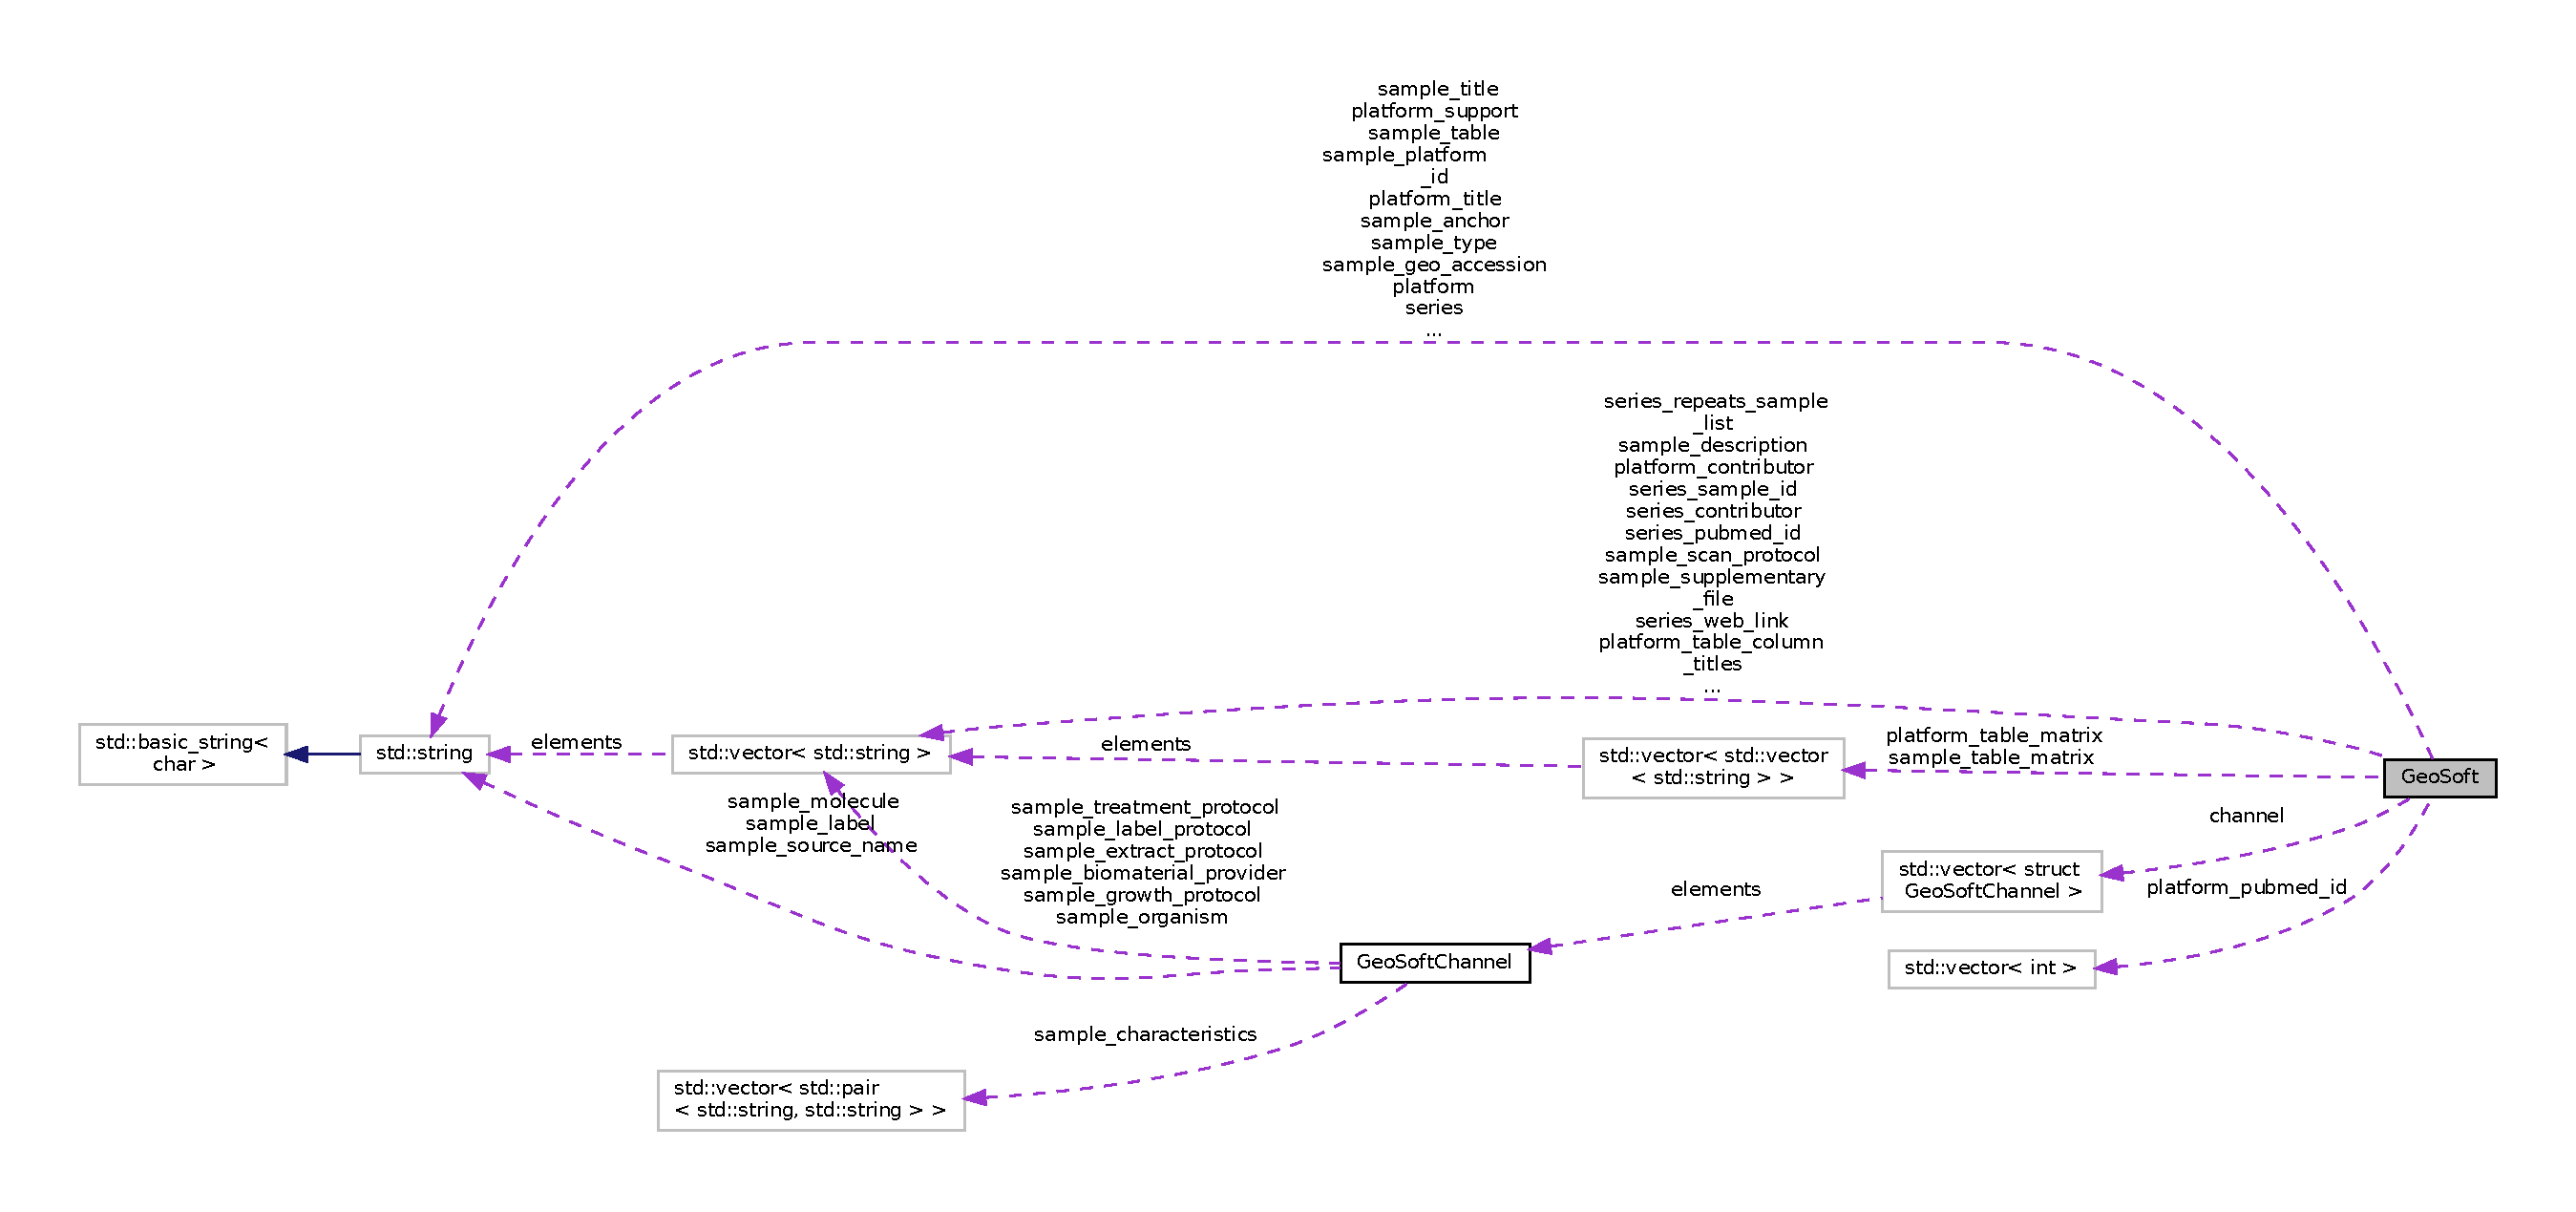
\includegraphics[width=350pt]{structGeoSoft__coll__graph}
\end{center}
\end{figure}
\subsection*{Public Attributes}
\begin{DoxyCompactItemize}
\item 
\mbox{\Hypertarget{structGeoSoft_a2c3a9073415ffd2788c0cc9db64ec1ea}\label{structGeoSoft_a2c3a9073415ffd2788c0cc9db64ec1ea}} 
std\+::string {\bfseries platform}
\item 
\mbox{\Hypertarget{structGeoSoft_ab4b8ef36843e6eddbf11e705a89b5c71}\label{structGeoSoft_ab4b8ef36843e6eddbf11e705a89b5c71}} 
std\+::string {\bfseries platform\+\_\+title}
\item 
\mbox{\Hypertarget{structGeoSoft_a6ecae76c8f3699f41c13d1bc355813f9}\label{structGeoSoft_a6ecae76c8f3699f41c13d1bc355813f9}} 
enum platform\+\_\+distribution\+\_\+enum {\bfseries platform\+\_\+distribution}
\item 
\mbox{\Hypertarget{structGeoSoft_aabc64301a99f64e66dd510c256d68dac}\label{structGeoSoft_aabc64301a99f64e66dd510c256d68dac}} 
enum platform\+\_\+technology\+\_\+enum {\bfseries platform\+\_\+technology}
\item 
\mbox{\Hypertarget{structGeoSoft_af6d445dc03c134cb7ce6644ef6f39664}\label{structGeoSoft_af6d445dc03c134cb7ce6644ef6f39664}} 
std\+::vector$<$ std\+::string $>$ {\bfseries platform\+\_\+organism}
\item 
\mbox{\Hypertarget{structGeoSoft_a7cf57fc715a1fb320ba1bda6c5181a3d}\label{structGeoSoft_a7cf57fc715a1fb320ba1bda6c5181a3d}} 
std\+::string {\bfseries platform\+\_\+manufacturer}
\item 
\mbox{\Hypertarget{structGeoSoft_a83ffef776fae057106e37af6c3e7062e}\label{structGeoSoft_a83ffef776fae057106e37af6c3e7062e}} 
std\+::vector$<$ std\+::string $>$ {\bfseries platform\+\_\+manufacture\+\_\+protocol}
\item 
\mbox{\Hypertarget{structGeoSoft_a2fca553de5ade9575c43c12b62cf478d}\label{structGeoSoft_a2fca553de5ade9575c43c12b62cf478d}} 
std\+::vector$<$ std\+::string $>$ {\bfseries platform\+\_\+catalog\+\_\+number}
\item 
\mbox{\Hypertarget{structGeoSoft_ad4e92e7eaca82851a9b98d8cb2badbf5}\label{structGeoSoft_ad4e92e7eaca82851a9b98d8cb2badbf5}} 
std\+::vector$<$ std\+::string $>$ {\bfseries platform\+\_\+web\+\_\+link}
\item 
\mbox{\Hypertarget{structGeoSoft_a3dc1c04870947c75e881d82c108dbfe0}\label{structGeoSoft_a3dc1c04870947c75e881d82c108dbfe0}} 
std\+::string {\bfseries platform\+\_\+support}
\item 
\mbox{\Hypertarget{structGeoSoft_ac6a2b4cea24979fbaae7b4035570d9fe}\label{structGeoSoft_ac6a2b4cea24979fbaae7b4035570d9fe}} 
std\+::string {\bfseries platform\+\_\+coating}
\item 
\mbox{\Hypertarget{structGeoSoft_a1c46744829230258c32d30dc4efaa78e}\label{structGeoSoft_a1c46744829230258c32d30dc4efaa78e}} 
std\+::string {\bfseries platform\+\_\+description}
\item 
\mbox{\Hypertarget{structGeoSoft_ae8b4d688d95191425854c2f45e656f35}\label{structGeoSoft_ae8b4d688d95191425854c2f45e656f35}} 
std\+::vector$<$ std\+::string $>$ {\bfseries platform\+\_\+contributor}
\item 
\mbox{\Hypertarget{structGeoSoft_ac1b47c9e117ea78e8a02eb027c2b0945}\label{structGeoSoft_ac1b47c9e117ea78e8a02eb027c2b0945}} 
std\+::vector$<$ int $>$ {\bfseries platform\+\_\+pubmed\+\_\+id}
\item 
\mbox{\Hypertarget{structGeoSoft_a1652bb9b56ddd9891d2e6d806e94685f}\label{structGeoSoft_a1652bb9b56ddd9891d2e6d806e94685f}} 
std\+::string {\bfseries platform\+\_\+geo\+\_\+accession}
\item 
\mbox{\Hypertarget{structGeoSoft_a21634a342e59fbc3f58e66a576c352c9}\label{structGeoSoft_a21634a342e59fbc3f58e66a576c352c9}} 
std\+::vector$<$ std\+::string $>$ {\bfseries platform\+\_\+table\+\_\+column\+\_\+titles}
\item 
\mbox{\Hypertarget{structGeoSoft_aff0f9540dd4c63379a518bb409feb189}\label{structGeoSoft_aff0f9540dd4c63379a518bb409feb189}} 
std\+::vector$<$ std\+::vector$<$ std\+::string $>$ $>$ {\bfseries platform\+\_\+table\+\_\+matrix}
\item 
\mbox{\Hypertarget{structGeoSoft_aec7ad1febe0db88501e7f11668daed16}\label{structGeoSoft_aec7ad1febe0db88501e7f11668daed16}} 
std\+::string {\bfseries sample}
\item 
\mbox{\Hypertarget{structGeoSoft_a3d684b518530bd8b72b343a2ed08241e}\label{structGeoSoft_a3d684b518530bd8b72b343a2ed08241e}} 
std\+::string {\bfseries sample\+\_\+title}
\item 
\mbox{\Hypertarget{structGeoSoft_aa8f183fa6ad9742d08ec14f6223798b6}\label{structGeoSoft_aa8f183fa6ad9742d08ec14f6223798b6}} 
std\+::vector$<$ std\+::string $>$ {\bfseries sample\+\_\+supplementary\+\_\+file}
\item 
\mbox{\Hypertarget{structGeoSoft_a5afad62e351fe888bd4ab89dd098b574}\label{structGeoSoft_a5afad62e351fe888bd4ab89dd098b574}} 
std\+::string {\bfseries sample\+\_\+table}
\item 
\mbox{\Hypertarget{structGeoSoft_a79286ccfa9c70a768dbaa4f4e6f7c780}\label{structGeoSoft_a79286ccfa9c70a768dbaa4f4e6f7c780}} 
std\+::vector$<$ struct \mbox{\hyperlink{structGeoSoftChannel}{Geo\+Soft\+Channel}} $>$ {\bfseries channel}
\item 
\mbox{\Hypertarget{structGeoSoft_a8422cb69c02d87824ffb177994d94b4f}\label{structGeoSoft_a8422cb69c02d87824ffb177994d94b4f}} 
std\+::vector$<$ std\+::string $>$ {\bfseries sample\+\_\+hyb\+\_\+protocol}
\item 
\mbox{\Hypertarget{structGeoSoft_a7505eeeb224cfbe96664aeb2c5bda0bb}\label{structGeoSoft_a7505eeeb224cfbe96664aeb2c5bda0bb}} 
std\+::vector$<$ std\+::string $>$ {\bfseries sample\+\_\+scan\+\_\+protocol}
\item 
\mbox{\Hypertarget{structGeoSoft_a6cfddc4e445a670797c93d6dafae0c8e}\label{structGeoSoft_a6cfddc4e445a670797c93d6dafae0c8e}} 
std\+::vector$<$ std\+::string $>$ {\bfseries sample\+\_\+data\+\_\+processing}
\item 
\mbox{\Hypertarget{structGeoSoft_a90bb6b0962cd6a5f77543fe7d8b0a745}\label{structGeoSoft_a90bb6b0962cd6a5f77543fe7d8b0a745}} 
std\+::vector$<$ std\+::string $>$ {\bfseries sample\+\_\+description}
\item 
\mbox{\Hypertarget{structGeoSoft_ab66635819f673343c594bd8feeab03e3}\label{structGeoSoft_ab66635819f673343c594bd8feeab03e3}} 
std\+::string {\bfseries sample\+\_\+platform\+\_\+id}
\item 
\mbox{\Hypertarget{structGeoSoft_a0d49a29c758d27e7f11dca8fe9f140ec}\label{structGeoSoft_a0d49a29c758d27e7f11dca8fe9f140ec}} 
std\+::string {\bfseries sample\+\_\+geo\+\_\+accession}
\item 
\mbox{\Hypertarget{structGeoSoft_a6a8d1f82bc86f6d7a41093909fa4a0e2}\label{structGeoSoft_a6a8d1f82bc86f6d7a41093909fa4a0e2}} 
std\+::string {\bfseries sample\+\_\+anchor}
\item 
\mbox{\Hypertarget{structGeoSoft_aeac2b5c7b8bc23ac8ee07bf8821b9ac0}\label{structGeoSoft_aeac2b5c7b8bc23ac8ee07bf8821b9ac0}} 
std\+::string {\bfseries sample\+\_\+type}
\item 
\mbox{\Hypertarget{structGeoSoft_ac83a62c8fb5d83be1852bae9aee0be89}\label{structGeoSoft_ac83a62c8fb5d83be1852bae9aee0be89}} 
int {\bfseries sample\+\_\+tag\+\_\+count}
\item 
\mbox{\Hypertarget{structGeoSoft_a47b2aea879efc78cdd23aa1671d85556}\label{structGeoSoft_a47b2aea879efc78cdd23aa1671d85556}} 
int {\bfseries sample\+\_\+tag\+\_\+length}
\item 
\mbox{\Hypertarget{structGeoSoft_a1390a600f62f6153880bf563111a2c23}\label{structGeoSoft_a1390a600f62f6153880bf563111a2c23}} 
std\+::vector$<$ std\+::string $>$ {\bfseries sample\+\_\+table\+\_\+columns}
\item 
\mbox{\Hypertarget{structGeoSoft_a9d11749ade3169e4cdb80dd7e555e879}\label{structGeoSoft_a9d11749ade3169e4cdb80dd7e555e879}} 
std\+::vector$<$ std\+::vector$<$ std\+::string $>$ $>$ {\bfseries sample\+\_\+table\+\_\+matrix}
\item 
\mbox{\Hypertarget{structGeoSoft_a9c7260ea7df5a3f59033194d4f22bc09}\label{structGeoSoft_a9c7260ea7df5a3f59033194d4f22bc09}} 
std\+::string {\bfseries series}
\item 
\mbox{\Hypertarget{structGeoSoft_a9d0674a961c4704dff2ebada0c57c375}\label{structGeoSoft_a9d0674a961c4704dff2ebada0c57c375}} 
std\+::string {\bfseries series\+\_\+title}
\item 
\mbox{\Hypertarget{structGeoSoft_a35169463cb42c03f8a5c06b7ed8fbabc}\label{structGeoSoft_a35169463cb42c03f8a5c06b7ed8fbabc}} 
std\+::vector$<$ std\+::string $>$ {\bfseries series\+\_\+summary}
\item 
\mbox{\Hypertarget{structGeoSoft_a122b99a56de67951c56a3cd1162df01a}\label{structGeoSoft_a122b99a56de67951c56a3cd1162df01a}} 
std\+::string {\bfseries series\+\_\+overall\+\_\+design}
\item 
\mbox{\Hypertarget{structGeoSoft_af27397c8407c2ae47c51ecde69c20ae1}\label{structGeoSoft_af27397c8407c2ae47c51ecde69c20ae1}} 
std\+::vector$<$ std\+::string $>$ {\bfseries series\+\_\+pubmed\+\_\+id}
\item 
\mbox{\Hypertarget{structGeoSoft_a96a19be316b4c7c8d81eb91de82b89d0}\label{structGeoSoft_a96a19be316b4c7c8d81eb91de82b89d0}} 
std\+::vector$<$ std\+::string $>$ {\bfseries series\+\_\+web\+\_\+link}
\item 
\mbox{\Hypertarget{structGeoSoft_aa2fb6ad5a800788e6a5d2cc31b300fdd}\label{structGeoSoft_aa2fb6ad5a800788e6a5d2cc31b300fdd}} 
std\+::vector$<$ std\+::string $>$ {\bfseries series\+\_\+contributor}
\item 
\mbox{\Hypertarget{structGeoSoft_a8dc23067efcf62394bfeab3198320710}\label{structGeoSoft_a8dc23067efcf62394bfeab3198320710}} 
std\+::vector$<$ std\+::string $>$ {\bfseries series\+\_\+variable}
\item 
\mbox{\Hypertarget{structGeoSoft_a7a428f2f45462f895ba231461484af57}\label{structGeoSoft_a7a428f2f45462f895ba231461484af57}} 
std\+::vector$<$ std\+::string $>$ {\bfseries series\+\_\+variable\+\_\+description}
\item 
\mbox{\Hypertarget{structGeoSoft_aaea6eba61373277dab0cea861f8ad15b}\label{structGeoSoft_aaea6eba61373277dab0cea861f8ad15b}} 
std\+::vector$<$ std\+::string $>$ {\bfseries series\+\_\+variable\+\_\+sample\+\_\+list}
\item 
\mbox{\Hypertarget{structGeoSoft_a54c0e3e994e01dc72664a3708d14ae16}\label{structGeoSoft_a54c0e3e994e01dc72664a3708d14ae16}} 
std\+::vector$<$ std\+::string $>$ {\bfseries series\+\_\+repeats}
\item 
\mbox{\Hypertarget{structGeoSoft_aa1bb0eb5c8436bf24d09d462843db6e5}\label{structGeoSoft_aa1bb0eb5c8436bf24d09d462843db6e5}} 
std\+::vector$<$ std\+::string $>$ {\bfseries series\+\_\+repeats\+\_\+sample\+\_\+list}
\item 
\mbox{\Hypertarget{structGeoSoft_a2e536d82e9a454cffdd09f1e41116d6f}\label{structGeoSoft_a2e536d82e9a454cffdd09f1e41116d6f}} 
std\+::vector$<$ std\+::string $>$ {\bfseries series\+\_\+sample\+\_\+id}
\item 
\mbox{\Hypertarget{structGeoSoft_a2b55873f4d70d00e58d01ee9f6dcce0d}\label{structGeoSoft_a2b55873f4d70d00e58d01ee9f6dcce0d}} 
std\+::string {\bfseries series\+\_\+geo\+\_\+accession}
\end{DoxyCompactItemize}


The documentation for this struct was generated from the following file\+:\begin{DoxyCompactItemize}
\item 
include/geo-\/soft.\+hpp\end{DoxyCompactItemize}

\hypertarget{structGeoSoftChannel}{}\section{Geo\+Soft\+Channel Struct Reference}
\label{structGeoSoftChannel}\index{Geo\+Soft\+Channel@{Geo\+Soft\+Channel}}


Collaboration diagram for Geo\+Soft\+Channel\+:\nopagebreak
\begin{figure}[H]
\begin{center}
\leavevmode
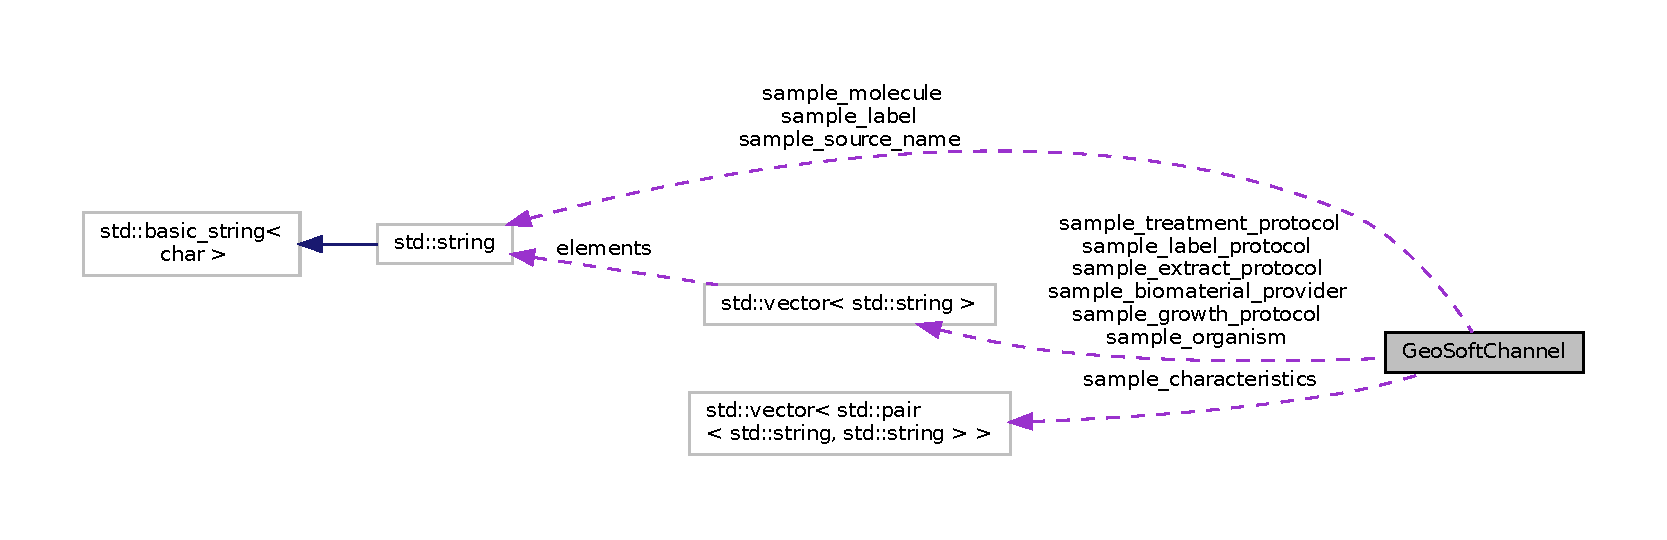
\includegraphics[width=350pt]{structGeoSoftChannel__coll__graph}
\end{center}
\end{figure}
\subsection*{Public Attributes}
\begin{DoxyCompactItemize}
\item 
\mbox{\Hypertarget{structGeoSoftChannel_afa7a7d494b8cae2bc86147747c8756ea}\label{structGeoSoftChannel_afa7a7d494b8cae2bc86147747c8756ea}} 
std\+::string {\bfseries sample\+\_\+source\+\_\+name}
\item 
\mbox{\Hypertarget{structGeoSoftChannel_a560b9467c399e867aca56e3c700c2c4d}\label{structGeoSoftChannel_a560b9467c399e867aca56e3c700c2c4d}} 
std\+::vector$<$ std\+::string $>$ {\bfseries sample\+\_\+organism}
\item 
\mbox{\Hypertarget{structGeoSoftChannel_af5daae70957d7d630af42615ec8e591a}\label{structGeoSoftChannel_af5daae70957d7d630af42615ec8e591a}} 
std\+::vector$<$ std\+::pair$<$ std\+::string, std\+::string $>$ $>$ {\bfseries sample\+\_\+characteristics}
\item 
\mbox{\Hypertarget{structGeoSoftChannel_abb3ff023351fdc307abeee1e67a48c00}\label{structGeoSoftChannel_abb3ff023351fdc307abeee1e67a48c00}} 
std\+::vector$<$ std\+::string $>$ {\bfseries sample\+\_\+biomaterial\+\_\+provider}
\item 
\mbox{\Hypertarget{structGeoSoftChannel_a04faf91b919c3b505dda80ed18fb0888}\label{structGeoSoftChannel_a04faf91b919c3b505dda80ed18fb0888}} 
std\+::vector$<$ std\+::string $>$ {\bfseries sample\+\_\+treatment\+\_\+protocol}
\item 
\mbox{\Hypertarget{structGeoSoftChannel_a85ff54508cabdf6461a6d9cf0087072a}\label{structGeoSoftChannel_a85ff54508cabdf6461a6d9cf0087072a}} 
std\+::vector$<$ std\+::string $>$ {\bfseries sample\+\_\+growth\+\_\+protocol}
\item 
\mbox{\Hypertarget{structGeoSoftChannel_ae33a3ee6e786ccda260dbbb74e4930ef}\label{structGeoSoftChannel_ae33a3ee6e786ccda260dbbb74e4930ef}} 
std\+::string {\bfseries sample\+\_\+molecule}
\item 
\mbox{\Hypertarget{structGeoSoftChannel_ae8eddd58a62be7cf23d8e3c218706a00}\label{structGeoSoftChannel_ae8eddd58a62be7cf23d8e3c218706a00}} 
std\+::vector$<$ std\+::string $>$ {\bfseries sample\+\_\+extract\+\_\+protocol}
\item 
\mbox{\Hypertarget{structGeoSoftChannel_a9380bc8aa2ad9a93901273e8d284ce66}\label{structGeoSoftChannel_a9380bc8aa2ad9a93901273e8d284ce66}} 
std\+::string {\bfseries sample\+\_\+label}
\item 
\mbox{\Hypertarget{structGeoSoftChannel_ace3d3dba88974a1f64a0da8a98a81a80}\label{structGeoSoftChannel_ace3d3dba88974a1f64a0da8a98a81a80}} 
std\+::vector$<$ std\+::string $>$ {\bfseries sample\+\_\+label\+\_\+protocol}
\end{DoxyCompactItemize}


The documentation for this struct was generated from the following file\+:\begin{DoxyCompactItemize}
\item 
include/geo-\/soft.\+hpp\end{DoxyCompactItemize}

\hypertarget{structmultithreadLoad}{}\section{multithread\+Load Struct Reference}
\label{structmultithreadLoad}\index{multithread\+Load@{multithread\+Load}}


Collaboration diagram for multithread\+Load\+:\nopagebreak
\begin{figure}[H]
\begin{center}
\leavevmode
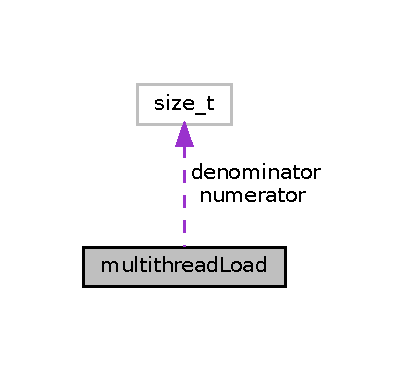
\includegraphics[width=195pt]{structmultithreadLoad__coll__graph}
\end{center}
\end{figure}
\subsection*{Public Attributes}
\begin{DoxyCompactItemize}
\item 
\mbox{\Hypertarget{structmultithreadLoad_a35b5fc855f655778297d6c0577f15237}\label{structmultithreadLoad_a35b5fc855f655778297d6c0577f15237}} 
size\+\_\+t {\bfseries numerator}
\item 
\mbox{\Hypertarget{structmultithreadLoad_a8ce86b198ddd084d472b32a84d31ee45}\label{structmultithreadLoad_a8ce86b198ddd084d472b32a84d31ee45}} 
size\+\_\+t {\bfseries denominator}
\item 
\mbox{\Hypertarget{structmultithreadLoad_a79b42a3037e255be1d9158a74bad2836}\label{structmultithreadLoad_a79b42a3037e255be1d9158a74bad2836}} 
void $\ast$ {\bfseries specifics}
\end{DoxyCompactItemize}


The documentation for this struct was generated from the following file\+:\begin{DoxyCompactItemize}
\item 
include/simple-\/thread-\/dispatch.\+hpp\end{DoxyCompactItemize}

\hypertarget{structrankHelpStruct}{}\section{rank\+Help\+Struct Struct Reference}
\label{structrankHelpStruct}\index{rank\+Help\+Struct@{rank\+Help\+Struct}}


Collaboration diagram for rank\+Help\+Struct\+:\nopagebreak
\begin{figure}[H]
\begin{center}
\leavevmode
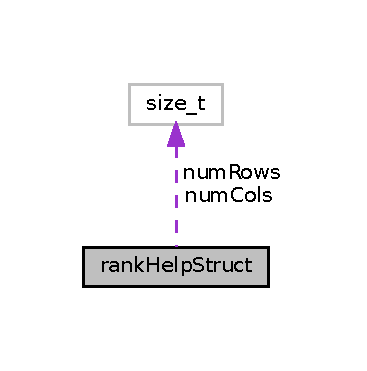
\includegraphics[width=176pt]{structrankHelpStruct__coll__graph}
\end{center}
\end{figure}
\subsection*{Public Attributes}
\begin{DoxyCompactItemize}
\item 
\mbox{\Hypertarget{structrankHelpStruct_a992a3fb809ed89ef5ed631f671535ca8}\label{structrankHelpStruct_a992a3fb809ed89ef5ed631f671535ca8}} 
cf64 $\ast$$\ast$ {\bfseries gene\+Corr\+Data}
\item 
\mbox{\Hypertarget{structrankHelpStruct_a51bf73dea1120f6bcc2e681c3fac0840}\label{structrankHelpStruct_a51bf73dea1120f6bcc2e681c3fac0840}} 
csize\+\_\+t {\bfseries num\+Rows}
\item 
\mbox{\Hypertarget{structrankHelpStruct_a1f20df966e9f704603296ddc4ca4860b}\label{structrankHelpStruct_a1f20df966e9f704603296ddc4ca4860b}} 
csize\+\_\+t {\bfseries num\+Cols}
\item 
\mbox{\Hypertarget{structrankHelpStruct_a2163f31046e19cb541d2108edcb12061}\label{structrankHelpStruct_a2163f31046e19cb541d2108edcb12061}} 
f64 $\ast$$\ast$ {\bfseries expression\+Data}
\end{DoxyCompactItemize}


The documentation for this struct was generated from the following files\+:\begin{DoxyCompactItemize}
\item 
src/pearson-\/correlation-\/matrix.\+cpp\item 
src/rank-\/matrix.\+cpp\item 
src/weighted-\/rank-\/correlation-\/matrix.\+cpp\end{DoxyCompactItemize}

\hypertarget{structSparseBitArrayRecord}{}\section{Sparse\+Bit\+Array\+Record Struct Reference}
\label{structSparseBitArrayRecord}\index{Sparse\+Bit\+Array\+Record@{Sparse\+Bit\+Array\+Record}}


Collaboration diagram for Sparse\+Bit\+Array\+Record\+:\nopagebreak
\begin{figure}[H]
\begin{center}
\leavevmode
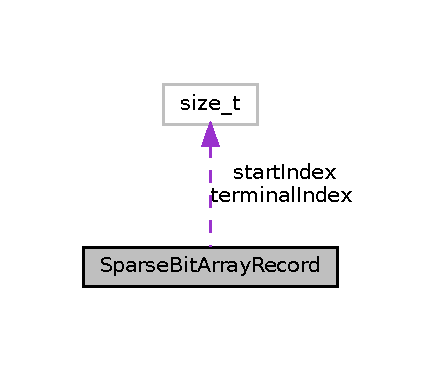
\includegraphics[width=210pt]{structSparseBitArrayRecord__coll__graph}
\end{center}
\end{figure}
\subsection*{Public Attributes}
\begin{DoxyCompactItemize}
\item 
\mbox{\Hypertarget{structSparseBitArrayRecord_af86795c8dc77f6dcd1c965df9f185003}\label{structSparseBitArrayRecord_af86795c8dc77f6dcd1c965df9f185003}} 
size\+\_\+t {\bfseries start\+Index}
\item 
\mbox{\Hypertarget{structSparseBitArrayRecord_a8b8a6007b9e20eba983e8a86840ae344}\label{structSparseBitArrayRecord_a8b8a6007b9e20eba983e8a86840ae344}} 
size\+\_\+t {\bfseries terminal\+Index}
\item 
\mbox{\Hypertarget{structSparseBitArrayRecord_aa7ff29c1e49eb345e7b66debf57a99a5}\label{structSparseBitArrayRecord_aa7ff29c1e49eb345e7b66debf57a99a5}} 
bit\+Array $\ast$ {\bfseries contents}
\end{DoxyCompactItemize}


The documentation for this struct was generated from the following file\+:\begin{DoxyCompactItemize}
\item 
src/sparse-\/bitpacked-\/array.\+c\end{DoxyCompactItemize}

\hypertarget{structSparseBitpackedArray}{}\section{Sparse\+Bitpacked\+Array Struct Reference}
\label{structSparseBitpackedArray}\index{Sparse\+Bitpacked\+Array@{Sparse\+Bitpacked\+Array}}


Collaboration diagram for Sparse\+Bitpacked\+Array\+:\nopagebreak
\begin{figure}[H]
\begin{center}
\leavevmode
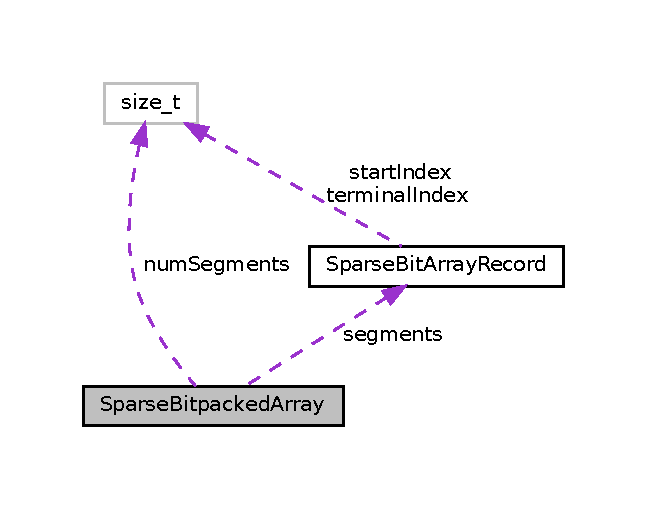
\includegraphics[width=311pt]{structSparseBitpackedArray__coll__graph}
\end{center}
\end{figure}
\subsection*{Public Attributes}
\begin{DoxyCompactItemize}
\item 
\mbox{\Hypertarget{structSparseBitpackedArray_a945b1ecd6c227bc2c71480ff4c4bdf62}\label{structSparseBitpackedArray_a945b1ecd6c227bc2c71480ff4c4bdf62}} 
size\+\_\+t {\bfseries num\+Segments}
\item 
\mbox{\Hypertarget{structSparseBitpackedArray_aae709970963dc4037e5c1be3d8dfe60b}\label{structSparseBitpackedArray_aae709970963dc4037e5c1be3d8dfe60b}} 
\mbox{\hyperlink{structSparseBitArrayRecord}{Sparse\+Bit\+Array\+Record}} $\ast$ {\bfseries segments}
\end{DoxyCompactItemize}


The documentation for this struct was generated from the following file\+:\begin{DoxyCompactItemize}
\item 
src/sparse-\/bitpacked-\/array.\+c\end{DoxyCompactItemize}

\hypertarget{structSuffixArray}{}\section{Suffix\+Array Struct Reference}
\label{structSuffixArray}\index{Suffix\+Array@{Suffix\+Array}}


Collaboration diagram for Suffix\+Array\+:\nopagebreak
\begin{figure}[H]
\begin{center}
\leavevmode
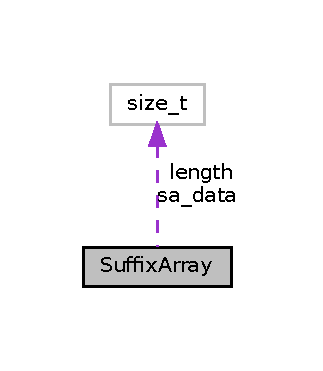
\includegraphics[width=155pt]{structSuffixArray__coll__graph}
\end{center}
\end{figure}
\subsection*{Public Attributes}
\begin{DoxyCompactItemize}
\item 
\mbox{\Hypertarget{structSuffixArray_aadf3610482051435eab01c4d41c139d9}\label{structSuffixArray_aadf3610482051435eab01c4d41c139d9}} 
const unsigned char $\ast$ {\bfseries sequence}
\item 
\mbox{\Hypertarget{structSuffixArray_ad11e732cc403a4ffe3ee304f9c0276b0}\label{structSuffixArray_ad11e732cc403a4ffe3ee304f9c0276b0}} 
bool {\bfseries do\+I\+Own\+Sequence}
\item 
\mbox{\Hypertarget{structSuffixArray_a3d1083953dbad8d1dcfc789c29c9dfd4}\label{structSuffixArray_a3d1083953dbad8d1dcfc789c29c9dfd4}} 
size\+\_\+t {\bfseries length}
\item 
\mbox{\Hypertarget{structSuffixArray_a97244e7297dcf96af1101094fae198c0}\label{structSuffixArray_a97244e7297dcf96af1101094fae198c0}} 
size\+\_\+t $\ast$ {\bfseries sa\+\_\+data}
\end{DoxyCompactItemize}


The documentation for this struct was generated from the following file\+:\begin{DoxyCompactItemize}
\item 
include/matching.\+hpp\end{DoxyCompactItemize}

\hypertarget{structSuffixArrayCaster}{}\section{Suffix\+Array\+Caster Struct Reference}
\label{structSuffixArrayCaster}\index{Suffix\+Array\+Caster@{Suffix\+Array\+Caster}}


Collaboration diagram for Suffix\+Array\+Caster\+:\nopagebreak
\begin{figure}[H]
\begin{center}
\leavevmode
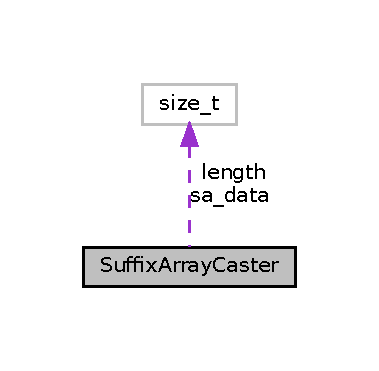
\includegraphics[width=182pt]{structSuffixArrayCaster__coll__graph}
\end{center}
\end{figure}
\subsection*{Public Attributes}
\begin{DoxyCompactItemize}
\item 
\mbox{\Hypertarget{structSuffixArrayCaster_a6256a8e22b3d80ad35bebd31cda53f0c}\label{structSuffixArrayCaster_a6256a8e22b3d80ad35bebd31cda53f0c}} 
unsigned char $\ast$ {\bfseries sequence}
\item 
\mbox{\Hypertarget{structSuffixArrayCaster_a9bf4ea707e59089a662b4170151395e0}\label{structSuffixArrayCaster_a9bf4ea707e59089a662b4170151395e0}} 
bool {\bfseries do\+I\+Own\+Sequence}
\item 
\mbox{\Hypertarget{structSuffixArrayCaster_a89b4f204e877c82ac0da03067d36333e}\label{structSuffixArrayCaster_a89b4f204e877c82ac0da03067d36333e}} 
size\+\_\+t {\bfseries length}
\item 
\mbox{\Hypertarget{structSuffixArrayCaster_adc11d827fd2d9207b98ea078a602e807}\label{structSuffixArrayCaster_adc11d827fd2d9207b98ea078a602e807}} 
size\+\_\+t $\ast$ {\bfseries sa\+\_\+data}
\end{DoxyCompactItemize}


The documentation for this struct was generated from the following file\+:\begin{DoxyCompactItemize}
\item 
include/matching.\+hpp\end{DoxyCompactItemize}

\hypertarget{structtauCorrHelpStructBruteForce}{}\section{tau\+Corr\+Help\+Struct\+Brute\+Force Struct Reference}
\label{structtauCorrHelpStructBruteForce}\index{tau\+Corr\+Help\+Struct\+Brute\+Force@{tau\+Corr\+Help\+Struct\+Brute\+Force}}


Collaboration diagram for tau\+Corr\+Help\+Struct\+Brute\+Force\+:\nopagebreak
\begin{figure}[H]
\begin{center}
\leavevmode
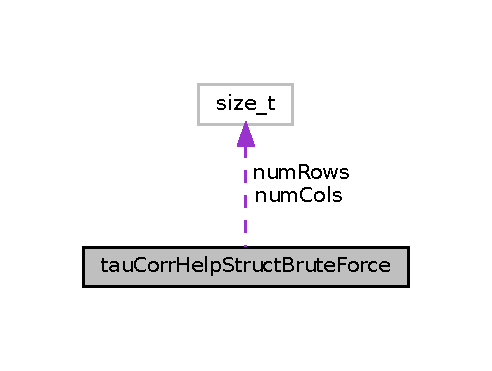
\includegraphics[width=236pt]{structtauCorrHelpStructBruteForce__coll__graph}
\end{center}
\end{figure}
\subsection*{Public Attributes}
\begin{DoxyCompactItemize}
\item 
\mbox{\Hypertarget{structtauCorrHelpStructBruteForce_abf5bf9e13f8fbaa9c51ac90519f58a66}\label{structtauCorrHelpStructBruteForce_abf5bf9e13f8fbaa9c51ac90519f58a66}} 
cf64 $\ast$$\ast$ {\bfseries expression\+Data}
\item 
\mbox{\Hypertarget{structtauCorrHelpStructBruteForce_aa761378aea37859cf7d7c61e8a077eba}\label{structtauCorrHelpStructBruteForce_aa761378aea37859cf7d7c61e8a077eba}} 
csize\+\_\+t {\bfseries num\+Rows}
\item 
\mbox{\Hypertarget{structtauCorrHelpStructBruteForce_abf804c94286f5cbd7a5eb5a9a1710abf}\label{structtauCorrHelpStructBruteForce_abf804c94286f5cbd7a5eb5a9a1710abf}} 
csize\+\_\+t {\bfseries num\+Cols}
\item 
\mbox{\Hypertarget{structtauCorrHelpStructBruteForce_ab2f1c28e7b57ae7c99cc4e9261bb8423}\label{structtauCorrHelpStructBruteForce_ab2f1c28e7b57ae7c99cc4e9261bb8423}} 
Upper\+Diagonal\+Square\+Matrix$<$ f64 $>$ $\ast$ {\bfseries results}
\end{DoxyCompactItemize}


The documentation for this struct was generated from the following file\+:\begin{DoxyCompactItemize}
\item 
src/kendall-\/correlation-\/matrix.\+cpp\end{DoxyCompactItemize}

\hypertarget{structtauCorrHelpStructCrossReference}{}\section{tau\+Corr\+Help\+Struct\+Cross\+Reference Struct Reference}
\label{structtauCorrHelpStructCrossReference}\index{tau\+Corr\+Help\+Struct\+Cross\+Reference@{tau\+Corr\+Help\+Struct\+Cross\+Reference}}


Collaboration diagram for tau\+Corr\+Help\+Struct\+Cross\+Reference\+:\nopagebreak
\begin{figure}[H]
\begin{center}
\leavevmode
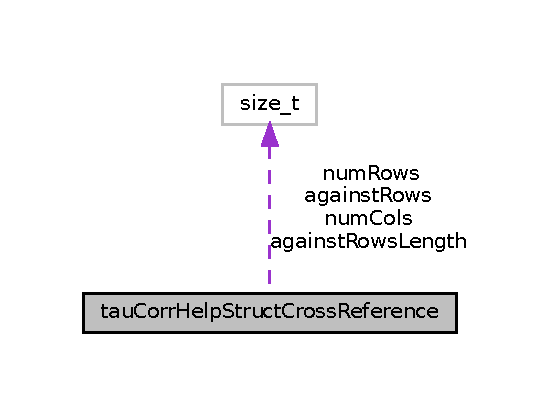
\includegraphics[width=265pt]{structtauCorrHelpStructCrossReference__coll__graph}
\end{center}
\end{figure}
\subsection*{Public Attributes}
\begin{DoxyCompactItemize}
\item 
\mbox{\Hypertarget{structtauCorrHelpStructCrossReference_a74acec2aba8e44d712aba0a6bd8dcb85}\label{structtauCorrHelpStructCrossReference_a74acec2aba8e44d712aba0a6bd8dcb85}} 
cf64 $\ast$$\ast$ {\bfseries expression\+Data}
\item 
\mbox{\Hypertarget{structtauCorrHelpStructCrossReference_a9250ad1ed1005faaa5be888052604ba3}\label{structtauCorrHelpStructCrossReference_a9250ad1ed1005faaa5be888052604ba3}} 
csize\+\_\+t {\bfseries num\+Rows}
\item 
\mbox{\Hypertarget{structtauCorrHelpStructCrossReference_a7077820518ebe7fe6109149f6f9549da}\label{structtauCorrHelpStructCrossReference_a7077820518ebe7fe6109149f6f9549da}} 
csize\+\_\+t {\bfseries num\+Cols}
\item 
\mbox{\Hypertarget{structtauCorrHelpStructCrossReference_a8f670f125a3faad96d4b7539dbf042c1}\label{structtauCorrHelpStructCrossReference_a8f670f125a3faad96d4b7539dbf042c1}} 
csize\+\_\+t $\ast$ {\bfseries against\+Rows}
\item 
\mbox{\Hypertarget{structtauCorrHelpStructCrossReference_ad33ae580179b325c9d8511a7aede598b}\label{structtauCorrHelpStructCrossReference_ad33ae580179b325c9d8511a7aede598b}} 
csize\+\_\+t {\bfseries against\+Rows\+Length}
\item 
\mbox{\Hypertarget{structtauCorrHelpStructCrossReference_a5a422c383ff264593bba2d58285d4e11}\label{structtauCorrHelpStructCrossReference_a5a422c383ff264593bba2d58285d4e11}} 
f64 $\ast$$\ast$ {\bfseries results}
\end{DoxyCompactItemize}


The documentation for this struct was generated from the following file\+:\begin{DoxyCompactItemize}
\item 
src/kendall-\/correlation-\/matrix.\+cpp\end{DoxyCompactItemize}

\hypertarget{structyy__buffer__state}{}\section{yy\+\_\+buffer\+\_\+state Struct Reference}
\label{structyy__buffer__state}\index{yy\+\_\+buffer\+\_\+state@{yy\+\_\+buffer\+\_\+state}}
\subsection*{Public Attributes}
\begin{DoxyCompactItemize}
\item 
\mbox{\Hypertarget{structyy__buffer__state_a4360acfb226a1fc240ab2be17dd6beda}\label{structyy__buffer__state_a4360acfb226a1fc240ab2be17dd6beda}} 
F\+I\+LE $\ast$ {\bfseries yy\+\_\+input\+\_\+file}
\item 
\mbox{\Hypertarget{structyy__buffer__state_a0d25458e69eb22207fc633a1255d099d}\label{structyy__buffer__state_a0d25458e69eb22207fc633a1255d099d}} 
char $\ast$ {\bfseries yy\+\_\+ch\+\_\+buf}
\item 
\mbox{\Hypertarget{structyy__buffer__state_a8435c3f786bbb55d21d0174e4cfc22a0}\label{structyy__buffer__state_a8435c3f786bbb55d21d0174e4cfc22a0}} 
char $\ast$ {\bfseries yy\+\_\+buf\+\_\+pos}
\item 
\mbox{\Hypertarget{structyy__buffer__state_a451d39697f006f3922c1f43cf79286b4}\label{structyy__buffer__state_a451d39697f006f3922c1f43cf79286b4}} 
int {\bfseries yy\+\_\+buf\+\_\+size}
\item 
\mbox{\Hypertarget{structyy__buffer__state_a06406208824817acfec2183b79080945}\label{structyy__buffer__state_a06406208824817acfec2183b79080945}} 
int {\bfseries yy\+\_\+n\+\_\+chars}
\item 
\mbox{\Hypertarget{structyy__buffer__state_a80ce2431c70dc4f89ced487f18449465}\label{structyy__buffer__state_a80ce2431c70dc4f89ced487f18449465}} 
int {\bfseries yy\+\_\+is\+\_\+our\+\_\+buffer}
\item 
\mbox{\Hypertarget{structyy__buffer__state_abf5c70eea75581b58c0ee7bd31b14490}\label{structyy__buffer__state_abf5c70eea75581b58c0ee7bd31b14490}} 
int {\bfseries yy\+\_\+is\+\_\+interactive}
\item 
\mbox{\Hypertarget{structyy__buffer__state_a9d60c60af6e1a6f69de16871fd64f85f}\label{structyy__buffer__state_a9d60c60af6e1a6f69de16871fd64f85f}} 
int {\bfseries yy\+\_\+at\+\_\+bol}
\item 
int \mbox{\hyperlink{structyy__buffer__state_a818e94bc9c766e683c60df1e9fd01199}{yy\+\_\+bs\+\_\+lineno}}
\item 
int \mbox{\hyperlink{structyy__buffer__state_a10c4fcd8be759e6bf11e6d3e8cdb0307}{yy\+\_\+bs\+\_\+column}}
\item 
\mbox{\Hypertarget{structyy__buffer__state_a63d2afbb1d79a3fc63df9e12626f827d}\label{structyy__buffer__state_a63d2afbb1d79a3fc63df9e12626f827d}} 
int {\bfseries yy\+\_\+fill\+\_\+buffer}
\item 
\mbox{\Hypertarget{structyy__buffer__state_a70fd925d37a2f0454fbd0def675d106c}\label{structyy__buffer__state_a70fd925d37a2f0454fbd0def675d106c}} 
int {\bfseries yy\+\_\+buffer\+\_\+status}
\end{DoxyCompactItemize}


\subsection{Member Data Documentation}
\mbox{\Hypertarget{structyy__buffer__state_a10c4fcd8be759e6bf11e6d3e8cdb0307}\label{structyy__buffer__state_a10c4fcd8be759e6bf11e6d3e8cdb0307}} 
\index{yy\+\_\+buffer\+\_\+state@{yy\+\_\+buffer\+\_\+state}!yy\+\_\+bs\+\_\+column@{yy\+\_\+bs\+\_\+column}}
\index{yy\+\_\+bs\+\_\+column@{yy\+\_\+bs\+\_\+column}!yy\+\_\+buffer\+\_\+state@{yy\+\_\+buffer\+\_\+state}}
\subsubsection{\texorpdfstring{yy\+\_\+bs\+\_\+column}{yy\_bs\_column}}
{\footnotesize\ttfamily int yy\+\_\+buffer\+\_\+state\+::yy\+\_\+bs\+\_\+column}

The column count. \mbox{\Hypertarget{structyy__buffer__state_a818e94bc9c766e683c60df1e9fd01199}\label{structyy__buffer__state_a818e94bc9c766e683c60df1e9fd01199}} 
\index{yy\+\_\+buffer\+\_\+state@{yy\+\_\+buffer\+\_\+state}!yy\+\_\+bs\+\_\+lineno@{yy\+\_\+bs\+\_\+lineno}}
\index{yy\+\_\+bs\+\_\+lineno@{yy\+\_\+bs\+\_\+lineno}!yy\+\_\+buffer\+\_\+state@{yy\+\_\+buffer\+\_\+state}}
\subsubsection{\texorpdfstring{yy\+\_\+bs\+\_\+lineno}{yy\_bs\_lineno}}
{\footnotesize\ttfamily int yy\+\_\+buffer\+\_\+state\+::yy\+\_\+bs\+\_\+lineno}

The line count. 

The documentation for this struct was generated from the following files\+:\begin{DoxyCompactItemize}
\item 
src/file-\/parsing/geo-\/soft/lex.\+yy.\+cc\item 
src/file-\/parsing/geo-\/soft/lex.\+yy.\+h\end{DoxyCompactItemize}

\hypertarget{structyy__trans__info}{}\section{yy\+\_\+trans\+\_\+info Struct Reference}
\label{structyy__trans__info}\index{yy\+\_\+trans\+\_\+info@{yy\+\_\+trans\+\_\+info}}
\subsection*{Public Attributes}
\begin{DoxyCompactItemize}
\item 
\mbox{\Hypertarget{structyy__trans__info_a5c9f61e770deef50bd4e697310342fe9}\label{structyy__trans__info_a5c9f61e770deef50bd4e697310342fe9}} 
flex\+\_\+int32\+\_\+t {\bfseries yy\+\_\+verify}
\item 
\mbox{\Hypertarget{structyy__trans__info_ae0715250c2bef261e596e77e0030f13e}\label{structyy__trans__info_ae0715250c2bef261e596e77e0030f13e}} 
flex\+\_\+int32\+\_\+t {\bfseries yy\+\_\+nxt}
\end{DoxyCompactItemize}


The documentation for this struct was generated from the following file\+:\begin{DoxyCompactItemize}
\item 
src/file-\/parsing/geo-\/soft/lex.\+yy.\+cc\end{DoxyCompactItemize}

\hypertarget{unionyyalloc}{}\section{yyalloc Union Reference}
\label{unionyyalloc}\index{yyalloc@{yyalloc}}


Collaboration diagram for yyalloc\+:\nopagebreak
\begin{figure}[H]
\begin{center}
\leavevmode
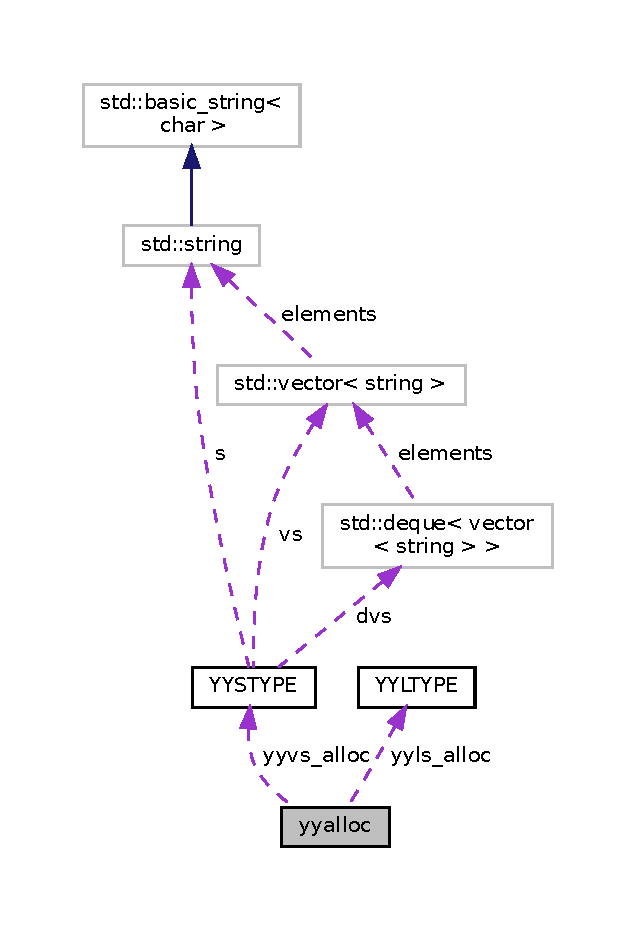
\includegraphics[width=305pt]{unionyyalloc__coll__graph}
\end{center}
\end{figure}
\subsection*{Public Attributes}
\begin{DoxyCompactItemize}
\item 
\mbox{\Hypertarget{unionyyalloc_a4800e0520a89a4789afa7b5d82197e65}\label{unionyyalloc_a4800e0520a89a4789afa7b5d82197e65}} 
yytype\+\_\+int16 {\bfseries yyss\+\_\+alloc}
\item 
\mbox{\Hypertarget{unionyyalloc_a9326f4fdc6f737a929444427836d8928}\label{unionyyalloc_a9326f4fdc6f737a929444427836d8928}} 
\mbox{\hyperlink{unionYYSTYPE}{Y\+Y\+S\+T\+Y\+PE}} {\bfseries yyvs\+\_\+alloc}
\item 
\mbox{\Hypertarget{unionyyalloc_a542e43248e6afac9af342c2f4e3162fc}\label{unionyyalloc_a542e43248e6afac9af342c2f4e3162fc}} 
\mbox{\hyperlink{structYYLTYPE}{Y\+Y\+L\+T\+Y\+PE}} {\bfseries yyls\+\_\+alloc}
\end{DoxyCompactItemize}


The documentation for this union was generated from the following file\+:\begin{DoxyCompactItemize}
\item 
src/file-\/parsing/geo-\/soft/geo-\/soft.\+tab.\+cc\end{DoxyCompactItemize}

\hypertarget{structyyguts__t}{}\section{yyguts\+\_\+t Struct Reference}
\label{structyyguts__t}\index{yyguts\+\_\+t@{yyguts\+\_\+t}}


Collaboration diagram for yyguts\+\_\+t\+:\nopagebreak
\begin{figure}[H]
\begin{center}
\leavevmode
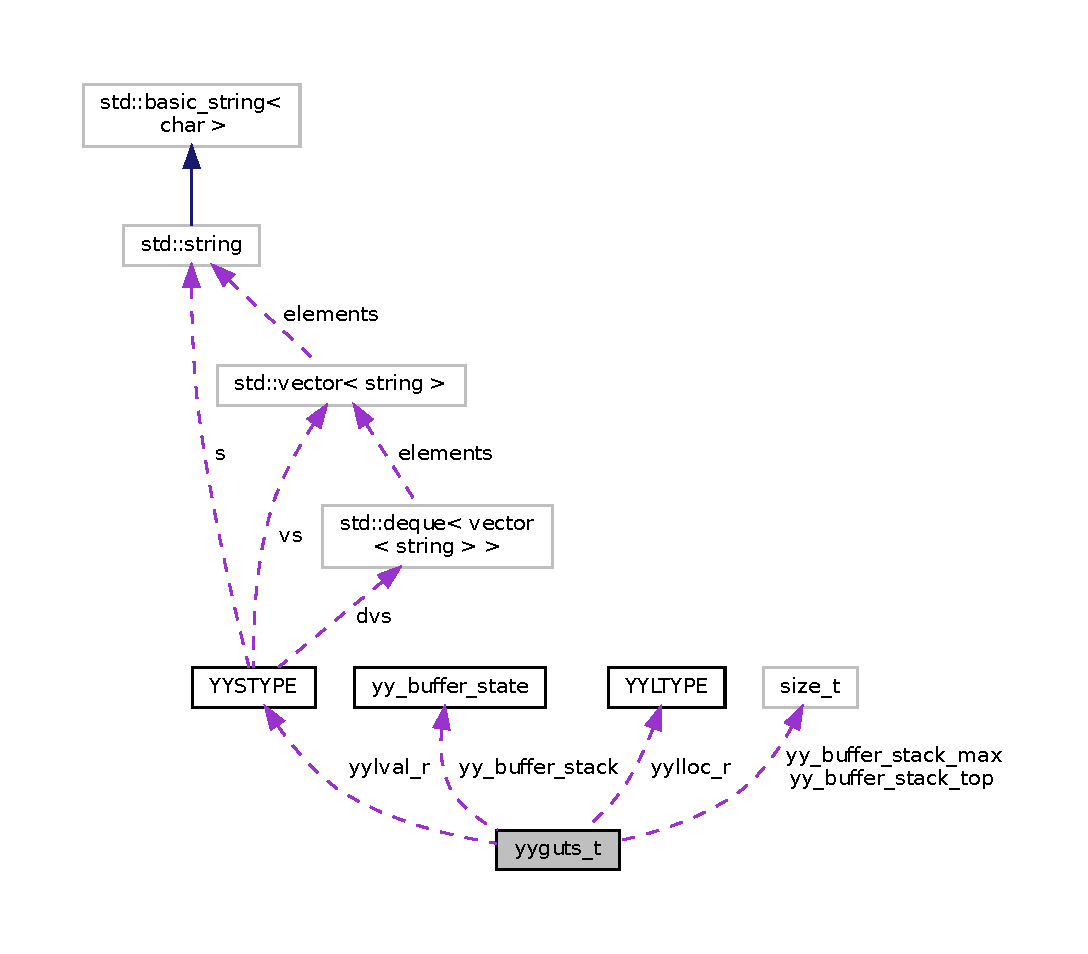
\includegraphics[width=350pt]{structyyguts__t__coll__graph}
\end{center}
\end{figure}
\subsection*{Public Attributes}
\begin{DoxyCompactItemize}
\item 
\mbox{\Hypertarget{structyyguts__t_aef05c0d6725a5214f6b30466f0b01c47}\label{structyyguts__t_aef05c0d6725a5214f6b30466f0b01c47}} 
Y\+Y\+\_\+\+E\+X\+T\+R\+A\+\_\+\+T\+Y\+PE {\bfseries yyextra\+\_\+r}
\item 
\mbox{\Hypertarget{structyyguts__t_a21f81ca100b12364a5095a37d1c6f650}\label{structyyguts__t_a21f81ca100b12364a5095a37d1c6f650}} 
F\+I\+LE $\ast$ {\bfseries yyin\+\_\+r}
\item 
\mbox{\Hypertarget{structyyguts__t_a436368a905aaf12e809e265749c74031}\label{structyyguts__t_a436368a905aaf12e809e265749c74031}} 
F\+I\+LE $\ast$ {\bfseries yyout\+\_\+r}
\item 
size\+\_\+t \mbox{\hyperlink{structyyguts__t_af92507d904af2fcd4509acde654a9850}{yy\+\_\+buffer\+\_\+stack\+\_\+top}}
\item 
size\+\_\+t \mbox{\hyperlink{structyyguts__t_a4435bb91e87f9988b096afc21386289a}{yy\+\_\+buffer\+\_\+stack\+\_\+max}}
\item 
\mbox{\hyperlink{structyy__buffer__state}{Y\+Y\+\_\+\+B\+U\+F\+F\+E\+R\+\_\+\+S\+T\+A\+TE}} $\ast$ \mbox{\hyperlink{structyyguts__t_ad0b9d576189d518a4482f20ed9b2a416}{yy\+\_\+buffer\+\_\+stack}}
\item 
\mbox{\Hypertarget{structyyguts__t_adde3f71374c223bbac47284824996e86}\label{structyyguts__t_adde3f71374c223bbac47284824996e86}} 
char {\bfseries yy\+\_\+hold\+\_\+char}
\item 
\mbox{\Hypertarget{structyyguts__t_a99c9218941829a6662d358422fd4184a}\label{structyyguts__t_a99c9218941829a6662d358422fd4184a}} 
int {\bfseries yy\+\_\+n\+\_\+chars}
\item 
\mbox{\Hypertarget{structyyguts__t_aba739bc731f0e9cbb0b6bdfca7930ebd}\label{structyyguts__t_aba739bc731f0e9cbb0b6bdfca7930ebd}} 
int {\bfseries yyleng\+\_\+r}
\item 
\mbox{\Hypertarget{structyyguts__t_ab1b9bcacb33aab1e02b625512bc0e221}\label{structyyguts__t_ab1b9bcacb33aab1e02b625512bc0e221}} 
char $\ast$ {\bfseries yy\+\_\+c\+\_\+buf\+\_\+p}
\item 
\mbox{\Hypertarget{structyyguts__t_abbef56b2d8359f6a15629c104f5dd030}\label{structyyguts__t_abbef56b2d8359f6a15629c104f5dd030}} 
int {\bfseries yy\+\_\+init}
\item 
\mbox{\Hypertarget{structyyguts__t_a8baf7d47fe53035d9bc2a9670795ff01}\label{structyyguts__t_a8baf7d47fe53035d9bc2a9670795ff01}} 
int {\bfseries yy\+\_\+start}
\item 
\mbox{\Hypertarget{structyyguts__t_a2daec411627700709ef2fd927e69627d}\label{structyyguts__t_a2daec411627700709ef2fd927e69627d}} 
int {\bfseries yy\+\_\+did\+\_\+buffer\+\_\+switch\+\_\+on\+\_\+eof}
\item 
\mbox{\Hypertarget{structyyguts__t_ad9e132dacc2904a8ae76c64c72e33795}\label{structyyguts__t_ad9e132dacc2904a8ae76c64c72e33795}} 
int {\bfseries yy\+\_\+start\+\_\+stack\+\_\+ptr}
\item 
\mbox{\Hypertarget{structyyguts__t_a35bedf1c17debd766565b99c39132eb4}\label{structyyguts__t_a35bedf1c17debd766565b99c39132eb4}} 
int {\bfseries yy\+\_\+start\+\_\+stack\+\_\+depth}
\item 
\mbox{\Hypertarget{structyyguts__t_af6e2e45a5fdba0f313c680b35da4292a}\label{structyyguts__t_af6e2e45a5fdba0f313c680b35da4292a}} 
int $\ast$ {\bfseries yy\+\_\+start\+\_\+stack}
\item 
\mbox{\Hypertarget{structyyguts__t_a84e01a3658729e9d69f79feb3faf1c99}\label{structyyguts__t_a84e01a3658729e9d69f79feb3faf1c99}} 
yy\+\_\+state\+\_\+type {\bfseries yy\+\_\+last\+\_\+accepting\+\_\+state}
\item 
\mbox{\Hypertarget{structyyguts__t_a46fb8d232ed375921af0b37caeeb67c4}\label{structyyguts__t_a46fb8d232ed375921af0b37caeeb67c4}} 
char $\ast$ {\bfseries yy\+\_\+last\+\_\+accepting\+\_\+cpos}
\item 
\mbox{\Hypertarget{structyyguts__t_aa9f13776b8d311e847cc7d974d49af4c}\label{structyyguts__t_aa9f13776b8d311e847cc7d974d49af4c}} 
int {\bfseries yylineno\+\_\+r}
\item 
\mbox{\Hypertarget{structyyguts__t_a5ad72d75ed6d693824fe7e02ce21118e}\label{structyyguts__t_a5ad72d75ed6d693824fe7e02ce21118e}} 
int {\bfseries yy\+\_\+flex\+\_\+debug\+\_\+r}
\item 
\mbox{\Hypertarget{structyyguts__t_aebaa731ad6cbe2411d104925e5bb3f2c}\label{structyyguts__t_aebaa731ad6cbe2411d104925e5bb3f2c}} 
char $\ast$ {\bfseries yytext\+\_\+r}
\item 
\mbox{\Hypertarget{structyyguts__t_a664a72171cc3e720fcb8120af9b72883}\label{structyyguts__t_a664a72171cc3e720fcb8120af9b72883}} 
int {\bfseries yy\+\_\+more\+\_\+flag}
\item 
\mbox{\Hypertarget{structyyguts__t_a683563bf4cd73f25b4c7b78579c1330e}\label{structyyguts__t_a683563bf4cd73f25b4c7b78579c1330e}} 
int {\bfseries yy\+\_\+more\+\_\+len}
\item 
\mbox{\Hypertarget{structyyguts__t_a55dbdcd46a36d34adcbfc29be44d10cf}\label{structyyguts__t_a55dbdcd46a36d34adcbfc29be44d10cf}} 
\mbox{\hyperlink{unionYYSTYPE}{Y\+Y\+S\+T\+Y\+PE}} $\ast$ {\bfseries yylval\+\_\+r}
\item 
\mbox{\Hypertarget{structyyguts__t_ab8e55a82f463922752514b4baf40621d}\label{structyyguts__t_ab8e55a82f463922752514b4baf40621d}} 
\mbox{\hyperlink{structYYLTYPE}{Y\+Y\+L\+T\+Y\+PE}} $\ast$ {\bfseries yylloc\+\_\+r}
\end{DoxyCompactItemize}


\subsection{Member Data Documentation}
\mbox{\Hypertarget{structyyguts__t_ad0b9d576189d518a4482f20ed9b2a416}\label{structyyguts__t_ad0b9d576189d518a4482f20ed9b2a416}} 
\index{yyguts\+\_\+t@{yyguts\+\_\+t}!yy\+\_\+buffer\+\_\+stack@{yy\+\_\+buffer\+\_\+stack}}
\index{yy\+\_\+buffer\+\_\+stack@{yy\+\_\+buffer\+\_\+stack}!yyguts\+\_\+t@{yyguts\+\_\+t}}
\subsubsection{\texorpdfstring{yy\+\_\+buffer\+\_\+stack}{yy\_buffer\_stack}}
{\footnotesize\ttfamily \mbox{\hyperlink{structyy__buffer__state}{Y\+Y\+\_\+\+B\+U\+F\+F\+E\+R\+\_\+\+S\+T\+A\+TE}}$\ast$ yyguts\+\_\+t\+::yy\+\_\+buffer\+\_\+stack}

Stack as an array. \mbox{\Hypertarget{structyyguts__t_a4435bb91e87f9988b096afc21386289a}\label{structyyguts__t_a4435bb91e87f9988b096afc21386289a}} 
\index{yyguts\+\_\+t@{yyguts\+\_\+t}!yy\+\_\+buffer\+\_\+stack\+\_\+max@{yy\+\_\+buffer\+\_\+stack\+\_\+max}}
\index{yy\+\_\+buffer\+\_\+stack\+\_\+max@{yy\+\_\+buffer\+\_\+stack\+\_\+max}!yyguts\+\_\+t@{yyguts\+\_\+t}}
\subsubsection{\texorpdfstring{yy\+\_\+buffer\+\_\+stack\+\_\+max}{yy\_buffer\_stack\_max}}
{\footnotesize\ttfamily size\+\_\+t yyguts\+\_\+t\+::yy\+\_\+buffer\+\_\+stack\+\_\+max}

capacity of stack. \mbox{\Hypertarget{structyyguts__t_af92507d904af2fcd4509acde654a9850}\label{structyyguts__t_af92507d904af2fcd4509acde654a9850}} 
\index{yyguts\+\_\+t@{yyguts\+\_\+t}!yy\+\_\+buffer\+\_\+stack\+\_\+top@{yy\+\_\+buffer\+\_\+stack\+\_\+top}}
\index{yy\+\_\+buffer\+\_\+stack\+\_\+top@{yy\+\_\+buffer\+\_\+stack\+\_\+top}!yyguts\+\_\+t@{yyguts\+\_\+t}}
\subsubsection{\texorpdfstring{yy\+\_\+buffer\+\_\+stack\+\_\+top}{yy\_buffer\_stack\_top}}
{\footnotesize\ttfamily size\+\_\+t yyguts\+\_\+t\+::yy\+\_\+buffer\+\_\+stack\+\_\+top}

index of top of stack. 

The documentation for this struct was generated from the following file\+:\begin{DoxyCompactItemize}
\item 
src/file-\/parsing/geo-\/soft/lex.\+yy.\+cc\end{DoxyCompactItemize}

\hypertarget{structYYLTYPE}{}\section{Y\+Y\+L\+T\+Y\+PE Struct Reference}
\label{structYYLTYPE}\index{Y\+Y\+L\+T\+Y\+PE@{Y\+Y\+L\+T\+Y\+PE}}
\subsection*{Public Attributes}
\begin{DoxyCompactItemize}
\item 
\mbox{\Hypertarget{structYYLTYPE_a50ad3435eaea74bcab6f1ae5fbaefd89}\label{structYYLTYPE_a50ad3435eaea74bcab6f1ae5fbaefd89}} 
int {\bfseries first\+\_\+line}
\item 
\mbox{\Hypertarget{structYYLTYPE_a3a556533babab1b9066fa9bdbb809210}\label{structYYLTYPE_a3a556533babab1b9066fa9bdbb809210}} 
int {\bfseries first\+\_\+column}
\item 
\mbox{\Hypertarget{structYYLTYPE_a3075f2bc3448df5d2a9f16d22bff2cc1}\label{structYYLTYPE_a3075f2bc3448df5d2a9f16d22bff2cc1}} 
int {\bfseries last\+\_\+line}
\item 
\mbox{\Hypertarget{structYYLTYPE_acf87f8c98686f286eaf700c4b62157b2}\label{structYYLTYPE_acf87f8c98686f286eaf700c4b62157b2}} 
int {\bfseries last\+\_\+column}
\end{DoxyCompactItemize}


The documentation for this struct was generated from the following files\+:\begin{DoxyCompactItemize}
\item 
src/file-\/parsing/geo-\/soft/geo-\/soft.\+tab.\+cc\item 
src/file-\/parsing/geo-\/soft/geo-\/soft.\+tab.\+hh\end{DoxyCompactItemize}

\hypertarget{unionYYSTYPE}{}\section{Y\+Y\+S\+T\+Y\+PE Union Reference}
\label{unionYYSTYPE}\index{Y\+Y\+S\+T\+Y\+PE@{Y\+Y\+S\+T\+Y\+PE}}


Collaboration diagram for Y\+Y\+S\+T\+Y\+PE\+:\nopagebreak
\begin{figure}[H]
\begin{center}
\leavevmode
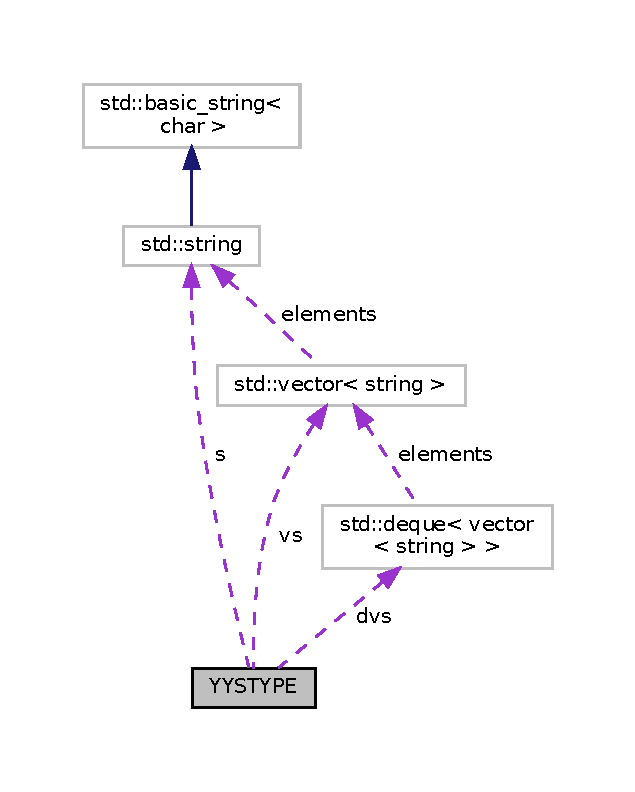
\includegraphics[width=305pt]{unionYYSTYPE__coll__graph}
\end{center}
\end{figure}
\subsection*{Public Attributes}
\begin{DoxyCompactItemize}
\item 
\mbox{\Hypertarget{unionYYSTYPE_a0bb334c57f831d5724188ac64f03e74a}\label{unionYYSTYPE_a0bb334c57f831d5724188ac64f03e74a}} 
vector$<$ string $>$ $\ast$ {\bfseries vs}
\item 
\mbox{\Hypertarget{unionYYSTYPE_a47f61089647b6a883ac504a9a877fc21}\label{unionYYSTYPE_a47f61089647b6a883ac504a9a877fc21}} 
int {\bfseries local\+\_\+int}
\item 
\mbox{\Hypertarget{unionYYSTYPE_a489e804ea5b945f50032f4e476b4b967}\label{unionYYSTYPE_a489e804ea5b945f50032f4e476b4b967}} 
deque$<$ vector$<$ string $>$ $>$ $\ast$ {\bfseries dvs}
\item 
\mbox{\Hypertarget{unionYYSTYPE_aa4c63d6e4455998c51a02b9991b64d6a}\label{unionYYSTYPE_aa4c63d6e4455998c51a02b9991b64d6a}} 
string $\ast$ {\bfseries s}
\end{DoxyCompactItemize}


The documentation for this union was generated from the following files\+:\begin{DoxyCompactItemize}
\item 
src/file-\/parsing/geo-\/soft/geo-\/soft.\+tab.\+cc\item 
src/file-\/parsing/geo-\/soft/geo-\/soft.\+tab.\+hh\end{DoxyCompactItemize}

%--- End generated contents ---

% Index
\backmatter
\newpage
\phantomsection
\clearemptydoublepage
\addcontentsline{toc}{chapter}{Index}
\printindex

\end{document}
